\section{Atomic Motion Extraction}
\label{sec:scene-hdp}

Tracking performance can be improved with the help of scene semantics.
For example, objects may have nonlinear changes in their sizes and speeds as they move due to camera perspectives,
and characterization of such non-linearity can regulate and benefit the tracking of the objects.
We propose an unsupervised framework, as shown in \ref{fig:scene-workflow}, to capture and exploit these constraints.
First, to capture global and long-range trajectories
with rich semantics,
local motion patterns of smaller units, such as fine-grained grids, are extracted (step 1).
We capture the local motion directions, which can be different but spatially interdependent across the grids, via a non-parametric topic model called \gls{hdp} \cite{yee2006hierarchical,wang2009unsupervised}.
For any scene, the model flexibly captures any local motion directions,
which are mixtures of base directions, without human presuming a universe of patterns.
Then, we synthesize global trajectories from the local patterns (step 2).
Specifically,
we adopt the trajectory finding algorithm from \cite{wang2009unsupervised} but improve it by:
(i) identifying multiple significant trajectories rather than a single one, and
(ii) sampling multiple possible instances from the same underlying trajectory to capture richer geometric information rather than a single line.
The sampled instances reveal key information for tracking:
(i) 
hotspots where vehicles enter and exit the scene; and
(ii) the extent in the direction perpendicular to the principal direction
(namely the direction from the starting to the ending point)
that will change nonlinearly but smoothly along that trajectory.
Lastly, we integrate the discovered hotspots and trajectories
in a tracking model as constraints to greatly reduce the false positives with improved or comparable false negatives.

%Third, more robustly identifying hotpots on a scene where vehicles are more likely to enter and exit the scene.
%integrate the semantic knowledge into an existing tracker, provide evidence for object's extry and exiting, and auxiliary motion and size constraints along tracking.
%We extend the results of the previous work \cite{wang2009unsupervised, zhao2013counting} to extract motion patterns by topic model and semantic features such as entry/exit area, size, and velocity statistics, finally integrate them with an existing tracker. Figure \ref{fig:workflow} gives an illustration of our flow work. Motion patterns are learned as \emph{visual topic}, where their distributions are fed to the post-processing unit, multiple lines following the movement of the visual topic are extracted, then the location and direction of the entry/exit areas are learned. 
%The learned topic model is used to do inference on new videos of the same camera, therefore, determine the assignment of the tracked object. 
%In the following part, we will briefly describe preliminary details for our method. Readers are referred to \cite{wang2009unsupervised, yee2006hierarchical} for more details about the topic model.
\begin{figure}
\centering
    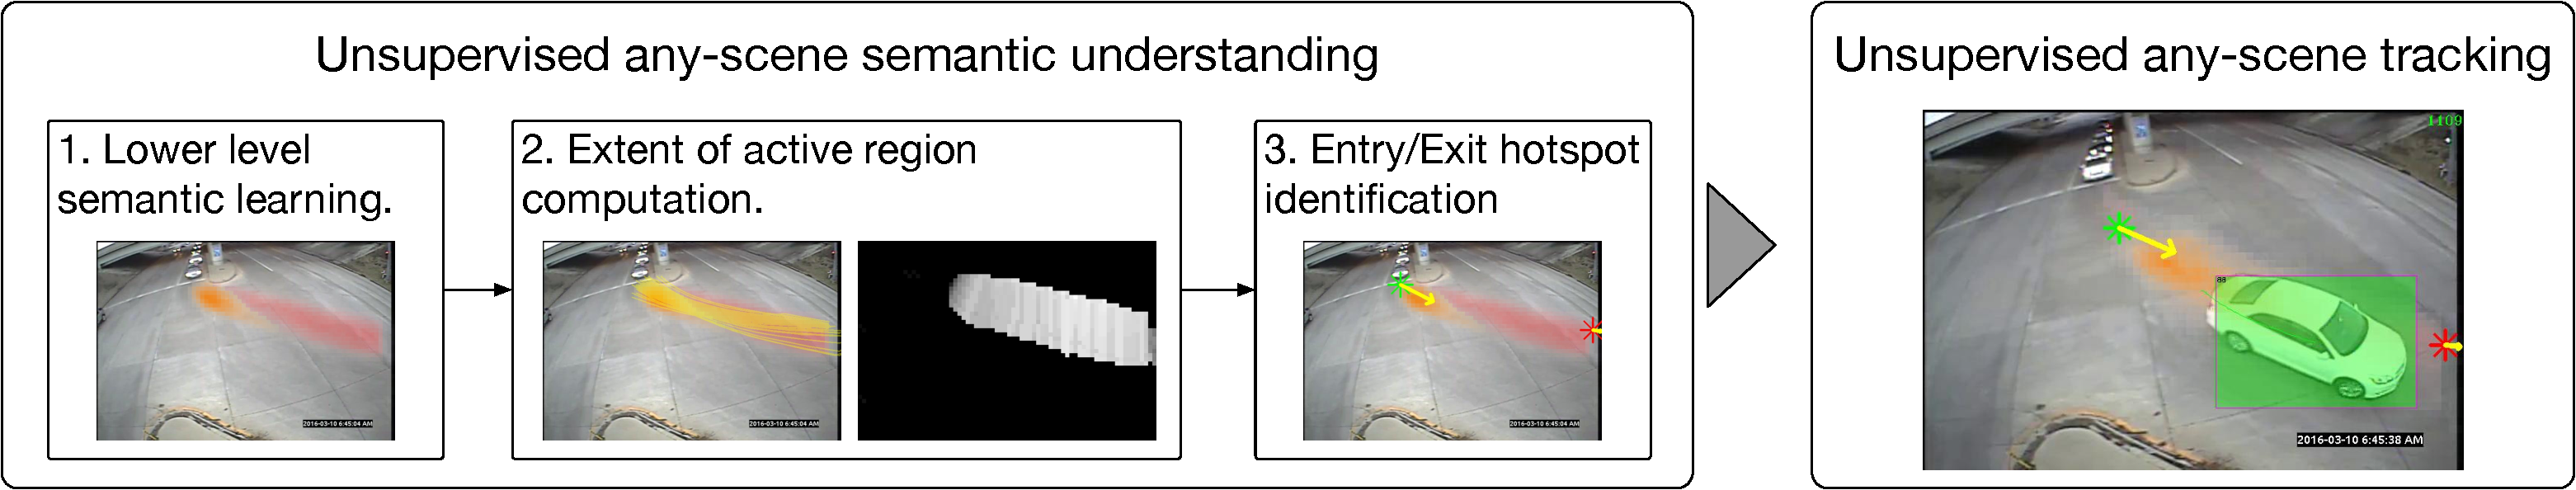
\includegraphics[width=\linewidth]{./img/scene_learning/workflow.pdf}
    \caption{System overview. The left corresponds to scene learning module: frequent motions are extracted in an unsupervised fashion, then the active regions where most objects move are learned on top of the motion result. Next, the entry/exit hotspot and their direction are extracted, describing how most objects enter and exit the scene. On the right, the semantic knowledge is applied to a tracker.}
    \label{fig:scene-workflow}
\end{figure}

\subsection{Non-parametric Clustering via \gls{hdp}}
\label{subsec:hdp-bag-of-words}
For general purpose of scene learning, lower-level representation could be a much more robust feature due to the difficulty of obtaining an accurate higher-level result, such as consistent object trajectories. Cluster of such low-level data as pixel movement could be an informative summary.
Inspired by the previous work \cite{wang2009unsupervised,kuettel2010s}, motion patterns are able to be learned by topic model, with a analogous bag-of-words representation to document classification.

Videos are processed as described in \ref{fig:scene-visual-doc}: first every frame is divided into small grids --- small enough to have consistent optical flow results. 
To distinguish different motions, optical flows of consecutive frames are quantized on $D$ directions after some simple filtering \cite{kalal2010forward}. 
Making an analogy with to document clustering, on a certain frame, each optical flow at a grid coordinate $(x, y)$ on a quantized direction is a \emph{visual word}.
If the frame is divided into $w\times h$ grids, the vocabulary will be $V = w\times h\times D$.
% To understand what a visual topic is, it is crucial to know how the video is represented in the topic model.
% Even the grid could be smaller and $D$ be even larger, the corresponding vocabulary size could also slow down the sampling algorithm of topic models. 
As shown in the middle column of \ref{fig:scene-visual-doc}, the videos are then split temporarily into short video clips. 
Each video clip has enough frames to contain a complete motion, at the same time, is not too long to have mixed motions. 
By counting the number of visual words on each grid and each quantized direction in every video clip, we have a bag-of-words representation of \emph{visual documents}. 
Similarly, a cluster trained from the video could be called \emph{visual topic}.
%Note that the bag-of-words representation treats each word independently. 
\begin{figure}
\centering
    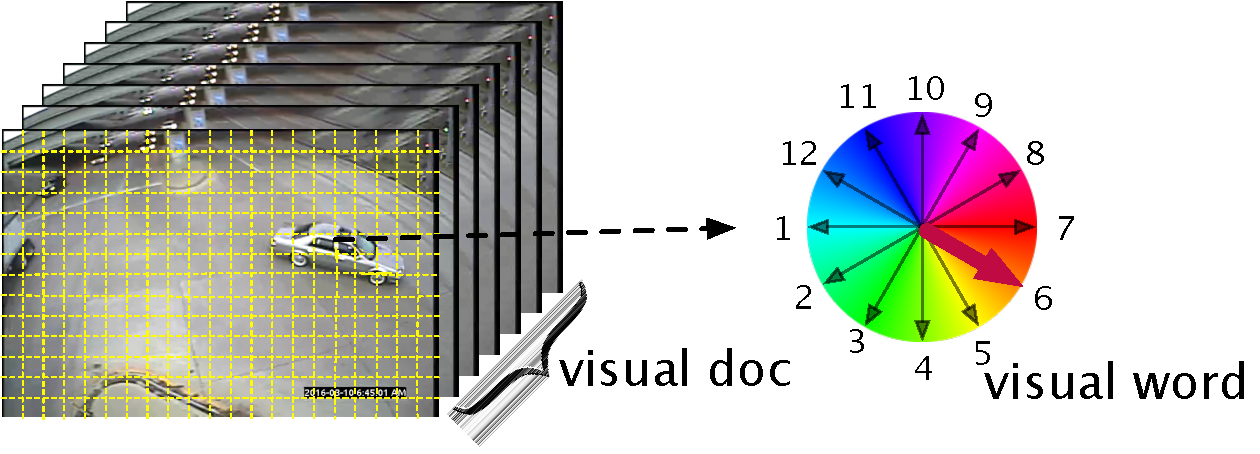
\includegraphics[width=0.8\linewidth]{./img/scene_learning/visual_doc.pdf}
    \caption{Left column illustrates the spatial and temporary quantization of video frames. The right shows a visual word obtained by discretizing the optical flow direction.}
    \label{fig:scene-visual-doc}
\end{figure}

% Using the bag-of-words representation, motions could be learned by any existing topic model method. 
% In most clustering methods, the number of clusters should be provided, and the results may vary according to the number of clusters. 
% Considering our goal to avoid unnecessary human input, we use the non-parametric model \gls{hdp} \cite{yee2006hierarchical} that required no specification of cluster numbers.
% It is a generalization of \gls{dp}. 
% In this model, the visual words are groups of observations, each exhibiting a mixed proportion of shared mixture components, also called “topics”. 
% An HDP is a two-level \gls{dp} with shared parameters. Each group $j$ is associated with a draw from a shared \gls{dp} whose base distribution is also a draw from the top-level \gls{dp}.
% \begin{align}
% G_0 & \sim DP(\gamma, H) \\
% G_j|G_0 & \sim DP(\alpha_0, G_0), \qquad \text{for each }j.
% \end{align}

% Here $j$ is the group index. 
% At the top-level, the distribution $G_0$ is drawn from a \gls{dp} with concentration parameter $\gamma$ and base distribution $H$. 
% The base distribution $H$ is a symmetric Dirichlet over the vocabulary simplex. Since the numbers drawn from a Dirichlet distribution sum up to 1, they are usually used as the parameter of a multinomial distribution. 
% Each atom is a distribution over the vocabulary, the atoms $\mathbf{\phi} = (\phi_k)_{k=1}^{\infty}$ are drawn independently $\phi_{k}\sim \text{Dirichlet}(\eta)$. 
% Simply speaking, $G_0$ is a discrete distribution over the atoms $\mathbf{\phi}$. 
% At the bottom level, $G_0$ is used as the base distribution to draw each group distribution $G_j$. 
% By such hierarchical definition, the atoms are shared among $G_j$, which makes sense that different documents may belong to the same topic.
% In this setting, a group is a visual document and the $i$th word is drawn from $j$th document $x_{ji}$ as follows,
% $$\theta_{ji}\sim G_j, \qquad x_{ji}\sim\text{Multi}(\theta_{ji}).$$

% Here $\theta_{ji}$ is the topic assignment of $x_{ji}$, which is associated with a multinomial distribution $\phi_{\theta_{ji}}$. 
% One could potentially have an infinite number of atoms. However, only a finite number of atoms/topics will be learned. 
% After Gibbs sampling, there is a multinomial distribution for each topic over the vocabulary where each word in a document has a topic assignment. 
% \ref{fig:scene-topics} visualizes those topics learned by HDP. 
% The color indicates the direction shown in the color wheel on the right and the lightness indicates the value of the multinomial at the corresponding cell. 
% To make it clear, a topic distribution is a multinomial distribution over the entire vocabulary, that is to say, each grid has $D$ values in the multinomial distribution. 
% For simplicity, we only visualize the maximal value on each grid. 
% The Figures show that HDP does a good job in summarizing the motions in the video, even without knowing any moving objects in the scene. For more details on Gibbs sampling, please see \cite{yee2006hierarchical}.
% With some relaxation of term use, we also call it \emph{the density on the main direction}.
Using the bag-of-words representation, motions could be learned by any existing topic model method. 
In most clustering methods, the number of clusters is required as an input, and the results usually vary accordingly. For complex videos, it is presumably hard for people to identify the number of major motions, therefore the non-parametric clustering method ---\gls{hdp} is used. 
It is a generalization of \gls{dp}, requiring no specification of the cluster number. 
In this model, visual words contain groups of observations, each exhibiting a mixed proportion of shared mixture components. 
The mixture components are learned in this model, also called ``topics''. 
More specifically, an \gls{hdp} is a two-level \gls{dp} with shared parameters. Each group $j$ is associated with a draw from a shared \gls{dp} whose base distribution is also a draw from the top-level \gls{dp}.
% In most clustering method, the results are sensitive to the number of clusters. Therefore, we naturally turn to Hierarchical Dirichlet Process (HDP), which is a non-parametric clustering method requiring no specification of cluster numbers. Figure \ref{fig:hdp} gives an graph illustration of HDP, Equation (\ref{eq:hdp}) gives mathematical formulation. We refer reader to \cite{yee2006hierarchical} for more details.
% \begin{figure} 
%     \center
%     \includegraphics[width=0.8\columnwidth]{./img/hdp.pdf}
%     \caption{Graph of HDP.}
%     \label{fig:hdp}
% \end{figure}
\begin{equation}    \label{eq:hdp}
\begin{aligned}    
    G_0 & \sim \text{DP}(\gamma, H) \\
    G_j|G_0 & \sim \text{DP}(\alpha_0, G_0), \text{for each } j,\\
\end{aligned}
\end{equation}
Here $j$ is the group index. At the top-level, the distribution $G_0$ is drawn from a \gls{dp} with concentration parameter $\gamma$ and base distribution $H$. 
The base distribution $H$ is a symmetric Dirichlet over the vocabulary simplex. 
Each atom is a distribution over the vocabulary, the atoms $\bm{\phi}=(\phi_k)^{\infty}_{k=1}$ are drawn independently $\phi_k \sim\text{Dirichlet}(\eta)$. Since the numbers drawn from a Dirichlet distribution sum up to 1, they are usually used as the parameters of a multinomial distribution. 
Simply speaking, $G_0$ is a discrete distribution over the atoms $\bm{\phi}$. 
At the bottom level, $G_0$ is used as the base distribution to draw each group distribution $G_j$, each is another multinomial distribution over the atoms $\bm{\phi}$. 
By such hierarchical definition, the atoms are shared among $G_j$, which makes sense that different documents may belong to the same topic.

In our setting, a group is a visual document and the $i$th word of the $j$th document $x_{ji}$ is drawn as follows:
\begin{equation}    \label{eq:multinomial}
\begin{aligned}
    \theta_{ji} = \phi_{z_{ji}}, \quad \theta_{ji}|G_j \sim G_j, \quad
    x_{ji}|\theta_{ji} \sim \text{Multi}(\theta_{ji})\\
\end{aligned}
\end{equation}
Here $z_{ji}$ is the topic assignment of $x_{ji}$, each word is associated with a multinomial distribution $\theta_{ji}$ according to its topic $z_{ji}$. 
We could potentially have an infinite number of atoms, however, only a finite number of atoms/topics will be learned. 
After Gibbs sampling, there is a multinomial distribution for each topic over the vocabulary where each word in a document has a topic assignment. 
In other word, words in the same document may belong to  \emph{different} topics. \ref{fig:scene-topics} visualizes those topics learned by HDP. 
The color indicates the direction shown in the color wheel on the right and the lightness indicates the value of the multinomial at the corresponding grid. 
The Figures show that HDP does a good job of summarizing the motions in the video, even without knowing any moving objects in the scene. 
For more details on the model and Gibbs sampling, please see \cite{yee2006hierarchical}. 
\begin{figure}
    \begin{subfigure}{0.32\linewidth}
        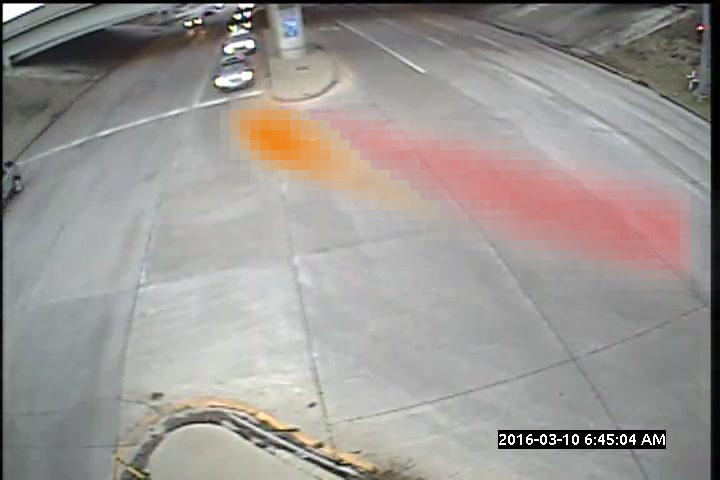
\includegraphics[width=\linewidth]{./img/scene_learning/topics/topic-1.jpg}
    \end{subfigure}%
    \begin{subfigure}{0.32\linewidth}
        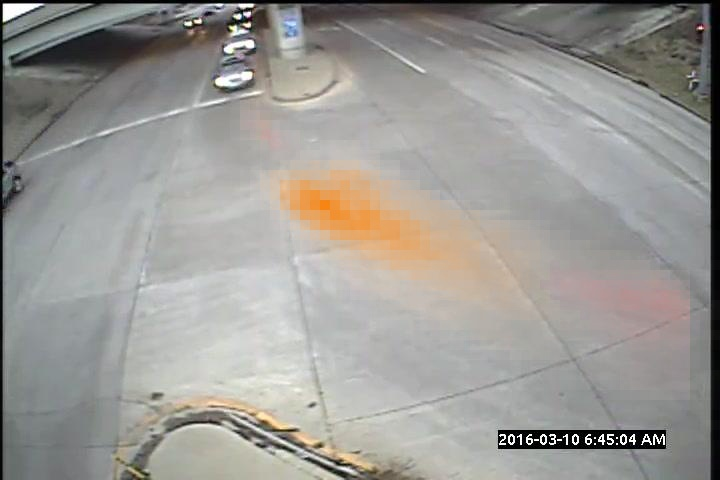
\includegraphics[width=\linewidth]{./img/scene_learning/topics/topic-3.jpg}
    \end{subfigure}%
    \begin{subfigure}{0.32\linewidth}
        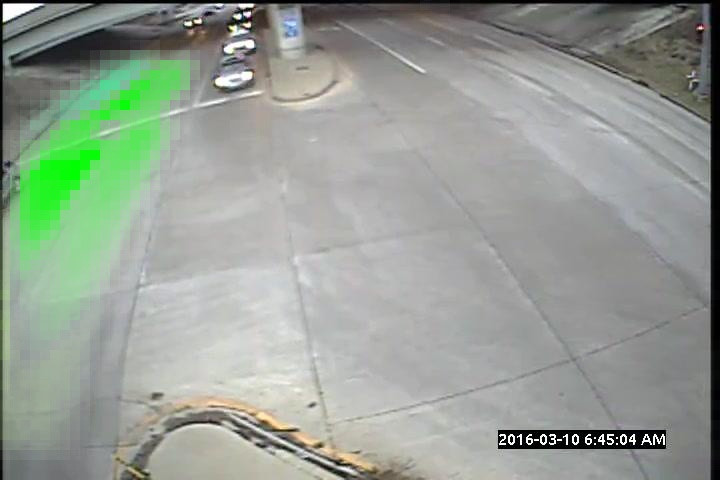
\includegraphics[width=\linewidth]{./img/scene_learning/topics/topic-0.jpg}
    \end{subfigure}%

    \begin{subfigure}{0.32\linewidth}
        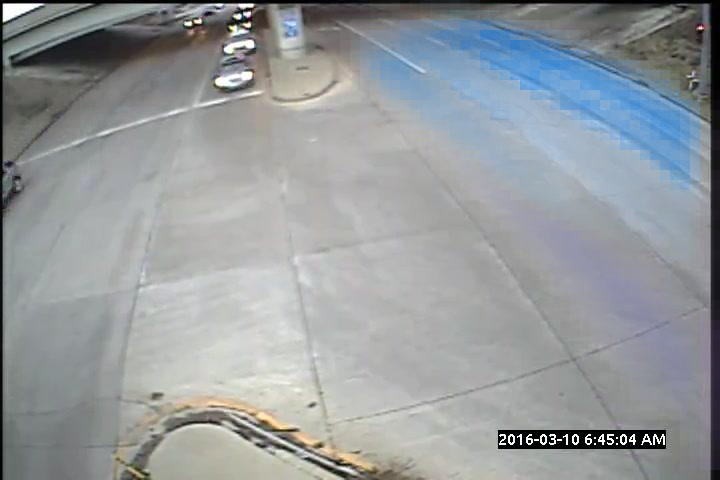
\includegraphics[width=\linewidth]{./img/scene_learning/topics/topic-2.jpg}
    \end{subfigure}%
    \begin{subfigure}{0.32\linewidth}
        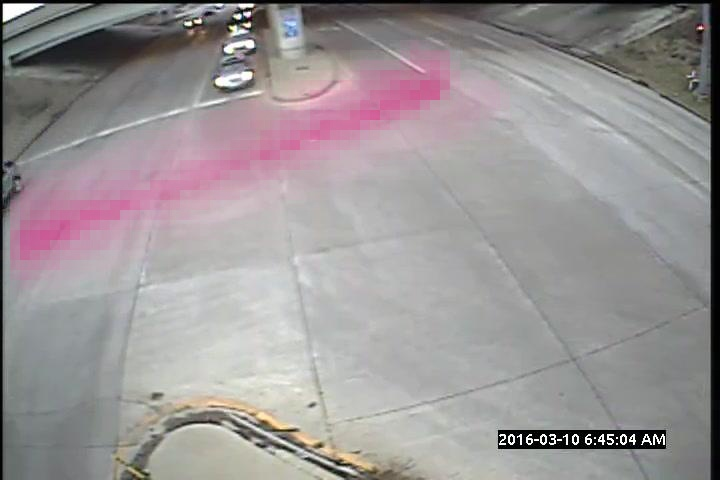
\includegraphics[width=\linewidth]{./img/scene_learning/topics/topic-4.jpg}
    \end{subfigure}%
    \hspace{0.08\linewidth}
    \begin{subfigure}{0.16\linewidth}
        
\includegraphics[width=\linewidth]{./img/scene_learning/color_wheel.png}
    \end{subfigure}
    \caption{Motions learned by HDP, colors indicate directions as the color wheel shows, the lightness indicate the magnitudes of the maximal probability values..}
    \label{fig:scene-topics}
\end{figure}
